% !TeX root = ../main.tex

\chapter{智能合约相关背景知识}

\section{智能合约中的常见漏洞}

\subsection{可重入 (Reentrancy)漏洞}

可重入漏洞是智能合约中最负盛名的漏洞。这个漏洞源于\emph{Solidity}语言上的一个特殊机制,像\emph{JavaScript}等语言一样,\emph{Solidity}语言有回调\codeff{fallback}函数。每个合约仅能有一个回调函数,并且这种函数没有参数,没有函数名,也不会返回任何的返回值。根据\emph{Solidity}的开发文档,这种函数只会在以下两种情况被触发:当合约收到函数调用但却没有符合的函数签名(函数的唯一标识符)时;当合约接收到任何数量的以太币,即发生交易时。前一种情况极少出现,而可重入攻击抓住的就是后面的那种情况。如果一个黑客妄图发动可重入攻击,他需要做的就是在自己的合约中编写一段恶意的回调函数,从而利用回调函数的特性反复记性转账操作,达到窃取以太币的目的。另一方面来说,如果被回调函数调用的函数中不包含转账语句,可重入漏洞也可利用重复调用,来造成拒绝服务(Denial of Service)攻击。因为在以太坊的体系中,每个合约都有一定的gas限制,gas会在合约的每一次调用、任何操作中消耗掉。如果重复调用一个函数,会不断消耗被调用函数所在合约的gas,待gas耗尽,合约不能提供任何的服务,也就达到了拒绝服务攻击的目的。在2016年,黑客借助可重入漏洞对DAO合约发动攻击,共盗取了价值数百万美元的以太币。

可重入漏洞在智能合约的漏洞中算是比较灵活的漏洞,其发动攻击的方式灵活多变,目前主要的防范方式是对函数调用者的身份进行检验,新版的\emph{Solidity}编译器也对有可重入风险的函数做出了提醒,但是仍有很多已经部署在以太坊平台上的合约存在可重入的风险,因此我们很重视可重入漏洞攻击模式的的分析,并会在之后的技术开发阶段对这种漏洞进行针对性的改进。

\subsection{意外异常 (Unexpected Revert)漏洞}

意外异常漏洞是由于EVM的异常处理机制引起的一种拒绝服务 (Denial of Service) 攻击。这种漏洞多出现于在for循环中进行的批量转账操作中。产生该漏洞的主要原因是,开发者使用\codeff{require}或者\codeff{assert}去检查写于\codeff{for}循环内的转账外部调用。如果其中一次转账发生错误,\codeff{require}函数将抛出异常,并终止整个交易过程,这将导致后面的地址无法正常进行转账业务。更进一步说,如果这样的转账错误是攻击者蓄意为之,那么这个意外异常漏洞就给了攻击者一个停止当前服务的机会。\emph{Solidity}研发团队不推荐也不建议开发者们在循环中进行任何的转账业务。

如下图\ref{fig:revert_vul}代码所示,在第5行,函数试图向\codeff{refundAddress}中存放的地址发送\codeff{ether}。该函数使用\codeff{send}函数,通过不断循环进行转账。同时,该函数也针对\codeff{send}函数用\codeff{require}进行了返回值检查。如果\codeff{refundAddress}中的任何一个地址发生转账错误,则该函数将停止运行,剩下的合约地址也没法正常进行转账业务。

\begin{figure}
\begin{minipage}[htb]{1.0\linewidth}
    \begin{lstlisting}
    address[] private refundAddresses;
    mapping (address => uint) public refunds;
    function refundAll() public {
            for(uint x; x < refundAddresses.length; x++) {
                require(refundAddresses[x].send(refunds[refundAddresses[x]]));
            }
    }
    \end{lstlisting}
    %\caption{test}
\end{minipage}
\vspace{-5mm}
\caption{意外异常调用漏洞示例代码}
\label{fig:revert_vul}
\end{figure}


\subsection{低级调用 (Unchecked Low-Level-Call)漏洞}

根据\emph{Solidity}的官方文档\cite{solidity-doc},\emph{Solidity}语言中的低级调用 (call, delegatecall, etc.) 在调用失败时会返回失败布尔值,这些布尔值如果没有被用户捕捉,用户就会错过调用的失败信息,从而造成智能合约功能的混乱。\emph{Solidity}语言经过数个版本的演化,推出了相对高级的内建外部调用 (transfer, send, etc.),这些高级调用会检查调用的返回值,并在发现调用失败时抛出异常。新部署的合约使用高级的外部调用,能避免使用低级外部调用带来的低级调用漏洞。然而,由于区块链语言的特性,智能合约一经部署,无法撤除。根据我们的统计和观察,在以太坊平台上,仍有大量仍在使用的合约在使用低级调用时,对外部调用的调用结果没有任何的检查措施,这些合约有受到低级调用漏洞攻击的危险。

\subsection{自毁 (Suicidal)漏洞}

\emph{Solidity}提供内建的自毁函数\codeff{selfdestruct()},这个函数需要输入一个地址类型的参数,任何调用这个函数的合约将停止当前合约功能,并把当前合约所有的余额转移到这个参数的地址。相比直接使用\codeff{send}函数进行余额转移,使用\codeff{selfdestruct}消耗的gas\footnote{以太坊上的每条指令都有的特定属性,表示这条指令消耗的资源多少,gas为0则停止任何服务}更少。

自毁函数给智能合约提供了方便的功能,但在实际的使用中,如果自毁函数没有被很好的限制,或对调用者的身份进行严格检查,就能造成漏洞攻击。如下面\ref{fig:suicidal_vul}代码所示,\codeff{suicidal}函数实现了简单的自毁函数功能,并通过传参来确定转移余额的目标地址。可是,函数的访问是公开的,任何一个访问该合约的用户都能调用这个自毁函数,并把自己的攻击地址作为余额的转账地址,造成自毁漏洞攻击。\emph{Solidity}研发团队在开发文档中提醒开发者要限制自毁函数的调用,并对调用者进行身份检查。

\begin{figure}
\begin{minipage}[htb]{1.0\linewidth}
    \begin{lstlisting}
    contract gamble{
        ...
        public suicidal(address target) public {
            selfdestruct(target);
        }
    }
    \end{lstlisting}
    %\caption{test}
\end{minipage}
\vspace{-5mm}
\caption{自毁漏洞示例代码}
\label{fig:suicidal_vul}
\end{figure}


\section{前沿智能合约分析工具}

\subsection{静态分析工具}

\subsubsection{传统静态分析工具}

传统静态分析是借助程序的中间语言(IR)、抽象语法树(AST)、控制流图(CFG)等等工具去分析程序特点的分析方法。静态分析方法的主要特点是覆盖率高(即能保证覆盖程序的尽可能多的执行路径),但准确率低。现有的传统静态分析工具代表如Slither,他的分析路径如下图\ref{fig:slither_proccess}所示:

\begin{figure}[h]
\vspace{+2mm}
  \centering
  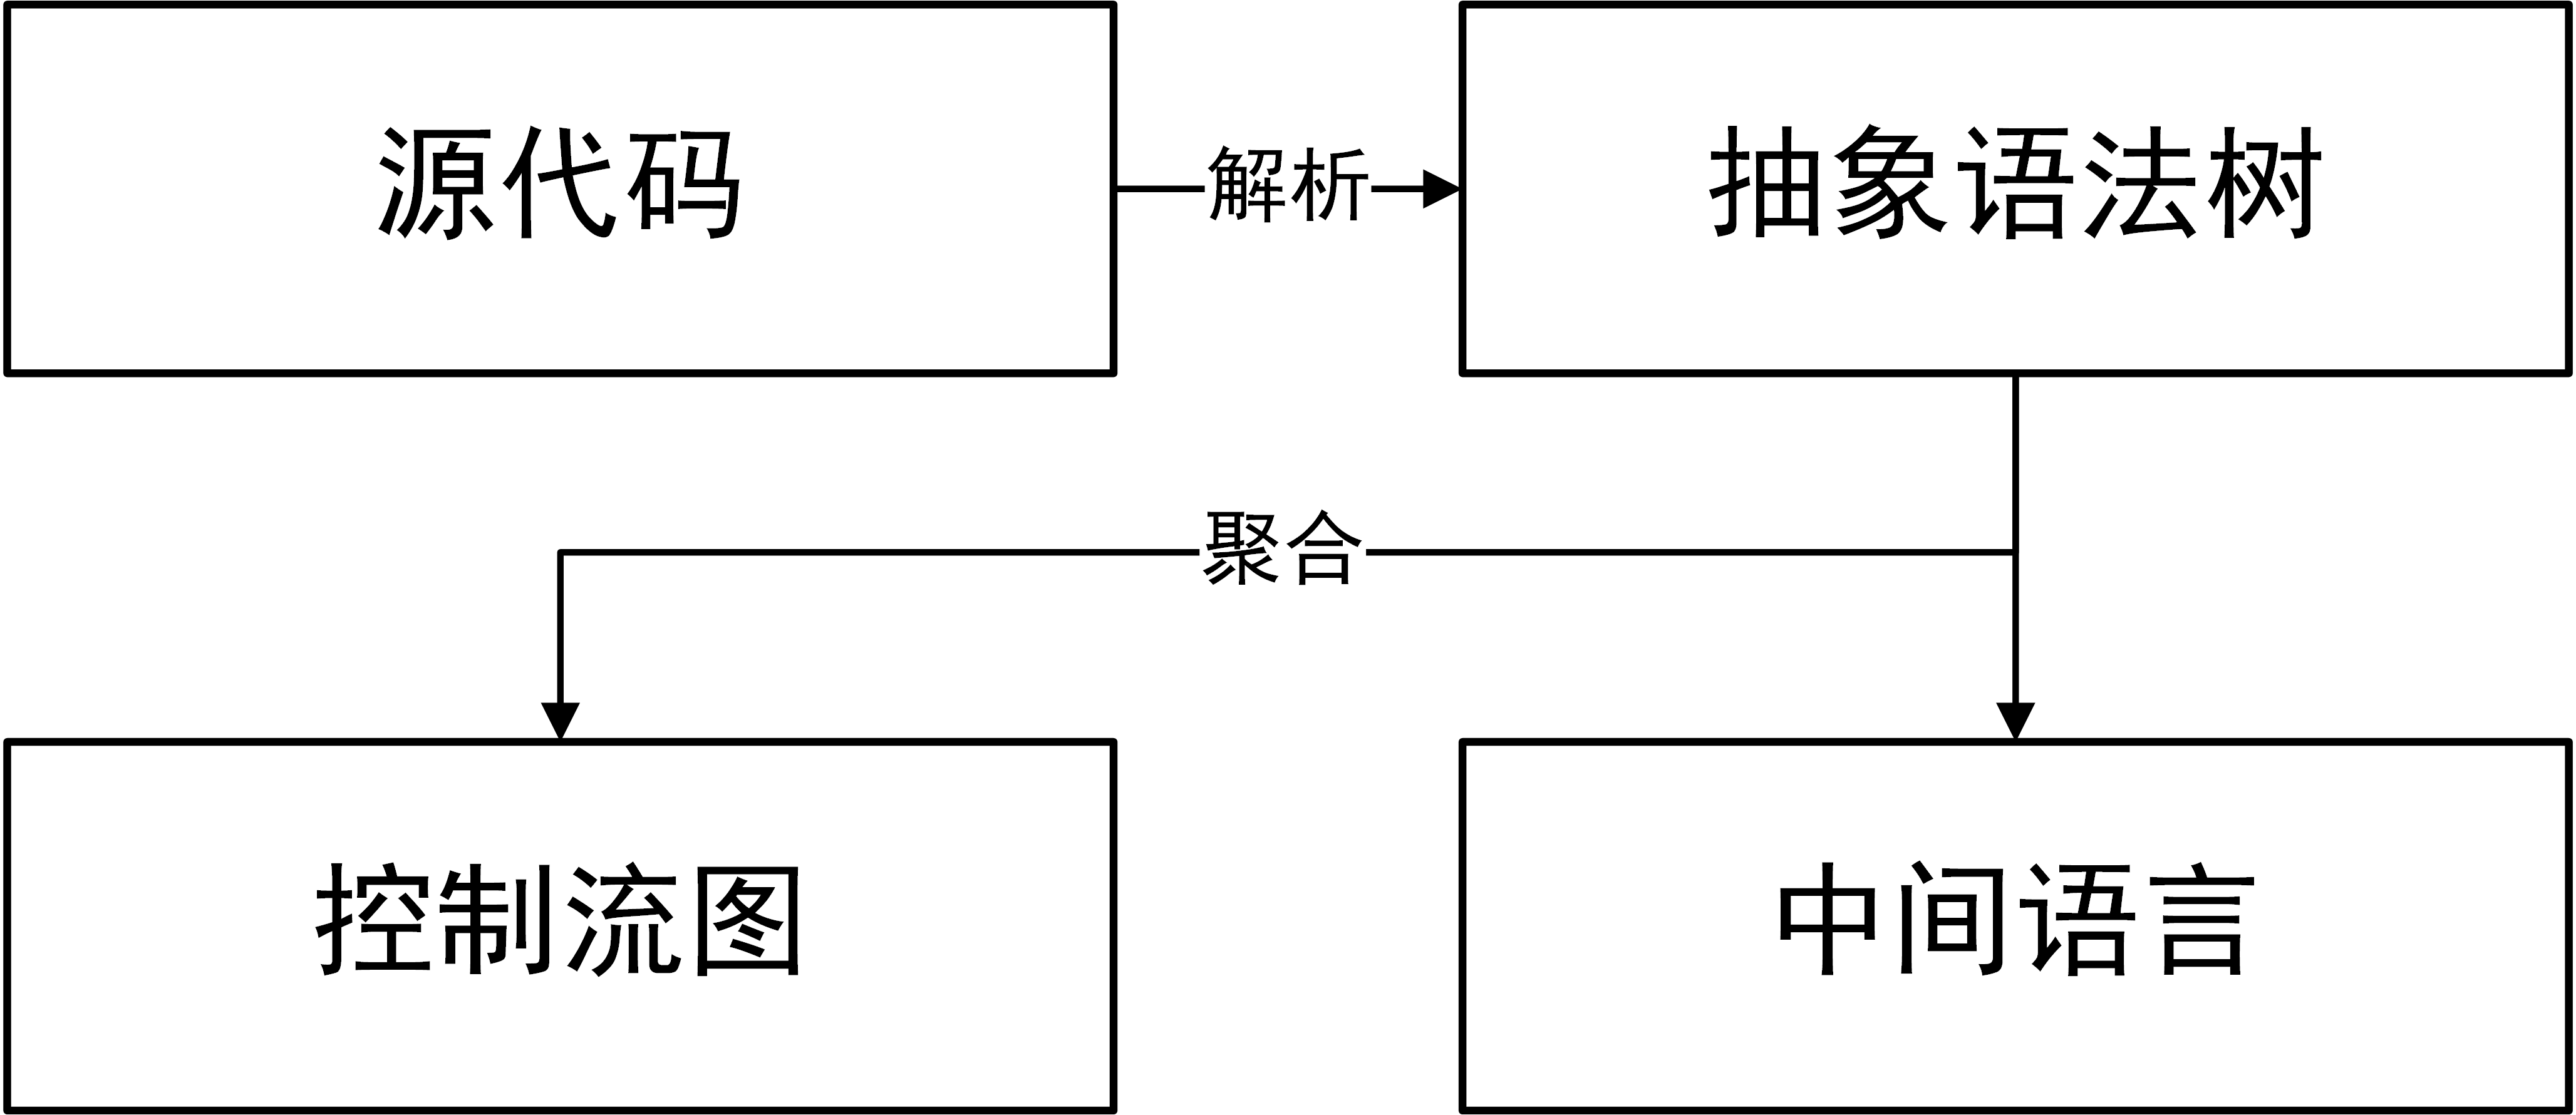
\includegraphics[width=0.55\textwidth]{figures/slither_process.png}
  \caption{\textsc{Slither}系统流程图}
  \vspace{-5mm}
  \label{fig:slither_proccess}
\end{figure}

以源代码作为输入,\textsc{Slither}首先借助\emph{Solidity}编译器将源代码经过编译,获取了程序的抽象语法树,再在AST上通过聚合、规则匹配的方式生成Slith中间语言(Intermediate Representation)和控制流图(Control Flow Graph)。由于\emph{Solidity}编译器生成了结构性强的抽象语法树(Abstract Syntax Tree),为分析提供了方便,故Slither能够在AST上如此顺利地实现IR和CFG的转换。其中,Slith IR是\textsc{Slither}的开发团队设计的一款中间语言,对源代码的常见操作做了不同程度的抽象。在以上所有步骤都完成之后,\textsc{Slither}再借助不同的探测器对生成的CFG进行探测。探测器中是\textsc{Slither}预先设定好的探测规则,如果在分析过程中发现和探测规则吻合的程序片段,探测器就会报告这个程序片段存在漏洞。故严格意义上来说,\textsc{Slither}是一款基于规则的漏洞检测软件。一方面来说,基于规则的设定提升了\textsc{Slither}的检测速度,也保证了它的可扩展性;另一方面,如果规则的制订不够合理,或者规则的分析程度不能做到抽象性和准确性的平衡,基于规则的检测方法就会带来很高的假正确率(False Positive Rate)。例如,\textsc{Slither}中针对可重入漏洞的检测规则如下图\ref{fig:slither_reentrancy_flow}所示:

\begin{figure}
\vspace{+2mm}
  \centering
  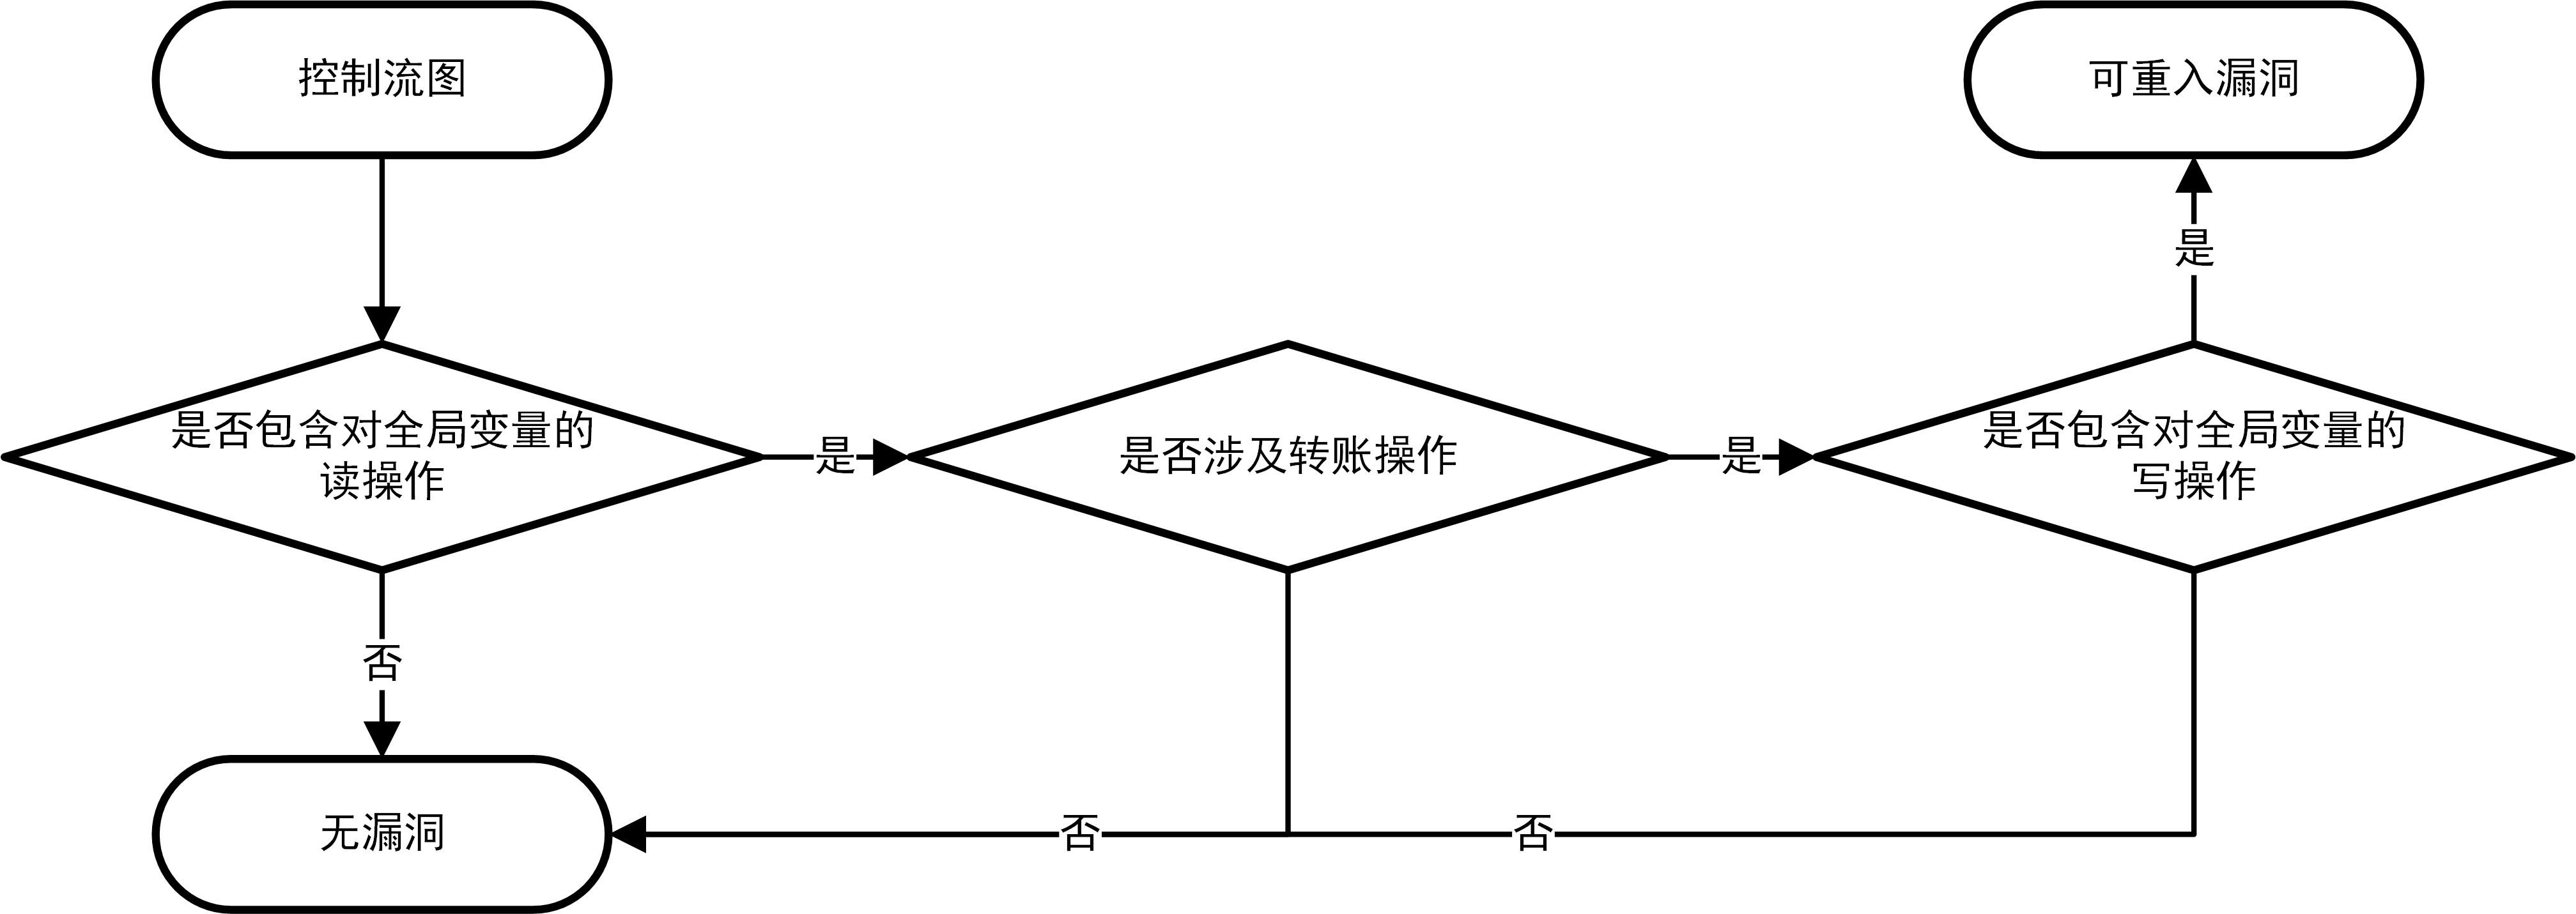
\includegraphics[width=0.9\textwidth]{figures/slither_reentrancy_flow.png}
  \caption{\textsc{Slihter}对可重入漏洞的判断逻辑}
  \label{fig:slither_reentrancy_flow}
\vspace{-5mm}
\end{figure}

在这个检测规则中,检测器逐一扫描CFG中的各个代码块,如果规则符合,就会报告漏洞。可重入漏洞的规则主要由三部分组成,其中任何一个条件不满足,都会被判断为清白的代码块,这三个条件包括:是否有对全局变量的读取操作、是否涉及交易过程、是否有对全局变量的写入操作。这个规则对可重入漏洞中的某一类型做出了准确地判断,但对其他新型变种可重入攻击,这个规则显得不够灵活。规则的修订过程是无止境的,基于规则的探测器不能保证漏洞检测的鲁棒性。如图\ref{fig:reentrancy_variant}所示,在这种潜在的可重入漏洞中,在安全的交易操作后面紧跟了一个危险的外部调用,这个危险的外部函数调用能触发对当前函数的二次访问。在我们看来,即使只重入了一次,只要造成经济损失,就要算作可重入漏洞。在我们观察\textsc{Slither}的内部原理后,我们发现\textsc{Slither}会漏掉类似的漏洞代码,它在安全的交易操作之后,没有发现对全局变量的写操作,这和\textsc{Slither}的检测规则相悖,故停止了检查,从而漏洞了紧随其后的危险外部调用。类似的例子还有很多,对于基于规则匹配的静态分析技术而言,不断修缮规则是一项长期的工作。

\begin{figure}
\vspace{+2mm}
  \centering
  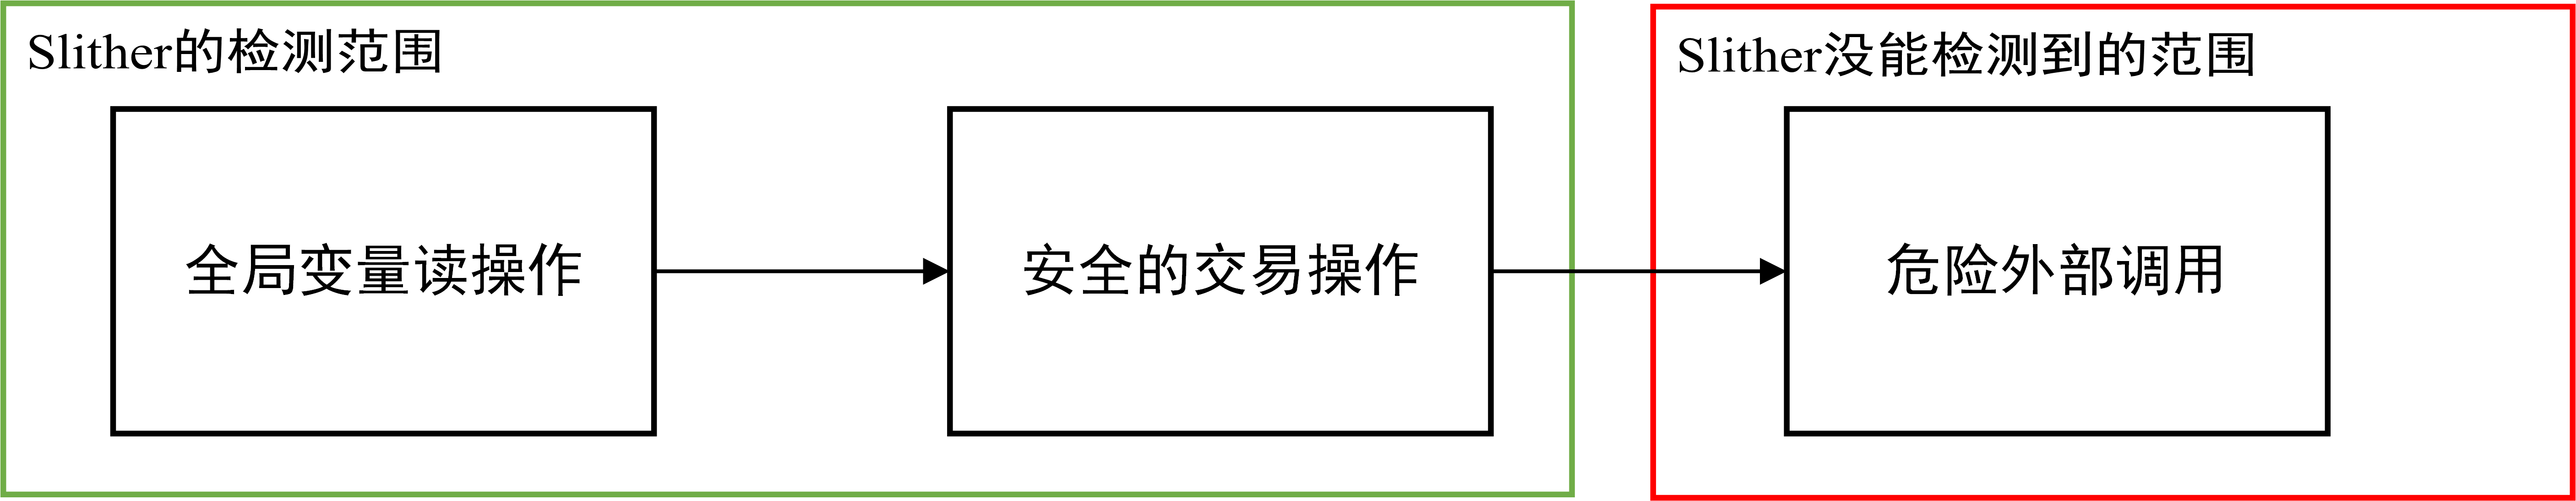
\includegraphics[width=0.9\textwidth]{figures/variant_reentrancy_pattern.png}
  \caption{\textsc{Slither}漏掉的潜在可重入漏洞}
  \label{fig:reentrancy_variant}
\vspace{-5mm}
\end{figure}



\subsubsection{符号执行分析工具}

符号执行分析工具主要将变量用符号进行标识,并利用约束求解器进行求解,来达到测试软件的墓地。符号执行工具没有像动态分析工具那样使用真实的用例观察软件的运行情况,而是利用约束求解技术或者其他技术代替真实值执行。在智能合约领域,代表的符号执行分析工具有\textsc{Oyente},\textsc{Oyente}的分析过程如下图\ref{fig:oyente_process}所示:

\begin{figure}
\vspace{+2mm}
  \centering
  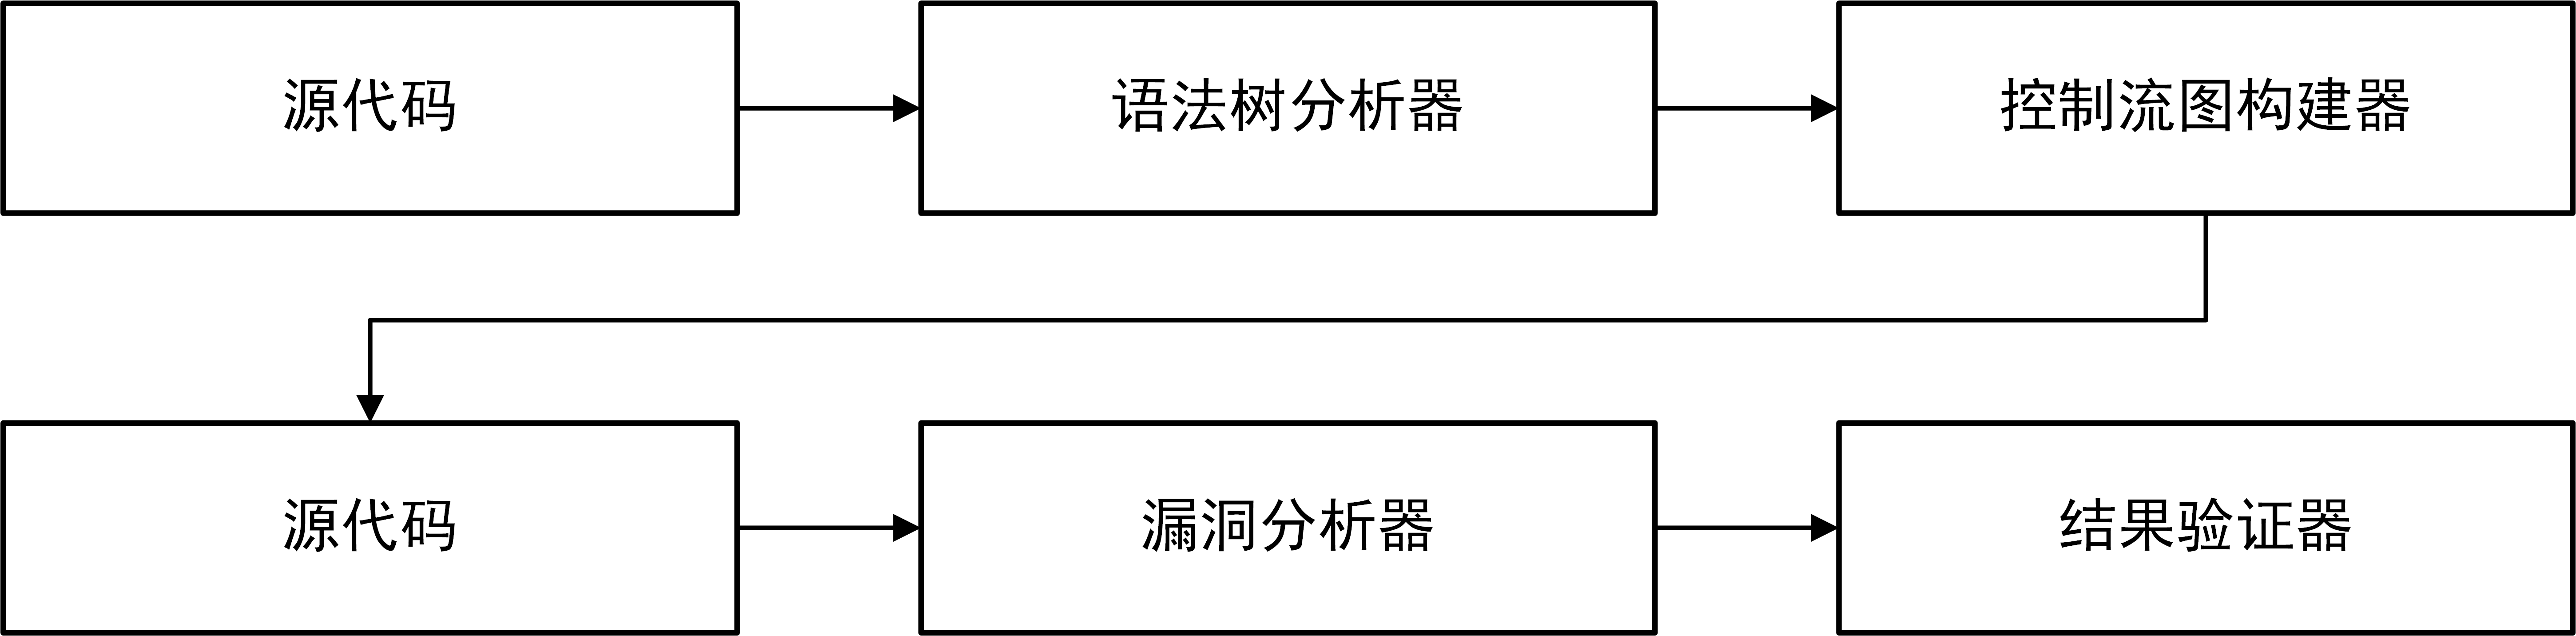
\includegraphics[width=0.9\textwidth]{figures/oyente_process.png}
  \caption{\textsc{Oyente}系统流程图}
  \label{fig:oyente_process}
\vspace{-5mm}
\end{figure}

\textsc{Oyente}的输入为源代码,再借助\emph{Solidity}编译器生成AST,进而生成CFG,再在CFG的基础上用Z3约束求解器进行符号执行,最后分析约束求解器的返回值并根据输出报告。\textsc{Oyente}的探测器在分析约束求解器的结果时,也用了基于规则的方法,如果约束求解器的结果和规则相符,则证明这个程序片段是有可能存在漏洞的。在执行流程的最后还有个验证器负责减少程序的误判。

作为典型的符号执行分析工具,\textsc{Oyente}充分体现了他的特点,它在同样的数据集上花费了近十倍于\textsc{Slither}的分析时间,耗时较长。遗憾的是,\textsc{Oyente}的结果并不是很好,输出的结果有很高的假正确率,我们推测是由于规则设置的不合理导致的。但不可否认的是,\textsc{Oyente}作为静态分析工具,能够分析一些传统静态分析工具无法分析的漏洞,比如整数的上溢、下溢,栈溢出等等,这些漏洞无法通过传统分析方法得出。

其他的分析工具如\textsc{Manticore},也采用了符号执行分析技术,这种技术带来了更高的精确度的同时也容易引入更差的性能表现。

\subsection{动态分析工具}

动态分析工具主要依赖于动态分析技术进行分析,这种技术使用测试用例作为输入,观察软件运行的状态(内存,耗时等等)和输出结果,进行分析并寻找程序漏洞。早期的动态分析技术多为黑盒测试,使用测试用例生成器不断产生测试用例,输入到软件中并观察结果。黑盒测试不依赖于软件本身的结构信息,只分析软件的运行状态及输入和输出之间的关系。早期的测试用例也是根据程序员本身的领域知识随机产生,由此也带来了测试用例测试效率低的问题——产生了大量的测试用例,却无法有效地测试到漏洞。为了解决以上问题,灰盒测试以及模糊测试诞生了。灰盒测试借助了静态分析技术来提高性能和表现,而模糊测试通过不同的标准来限制测试用例的数量,追求用最少的测试用例达到最高的测试效果。传统的模糊测试主要以程序的覆盖率作为标准,来引导整个测试过程,并采用了基于模型的或基于突变的测试用例生成器,解决了黑盒测试的主要问题,提高了测试效率。

在\emph{Solidity}这门语言上,静态分析工具有一定的局限性。例如,对于复杂的控制流关系,静态分析技术无法保证漏洞的触发问题,即虽然静态技术能保证很高的路径覆盖率,却不能保证检测到的漏洞能触发。\emph{Solidity}语言实现的智能合约,多数功能简单,控制流图相比传统的Linux软件要小很多,但即使在这样的软件上,静态分析也不能打到完美的效果。为此,在某些场景下,需要结合动态分析技术进行分析。当下前沿的动态分析工具有\textsc{ContractFuzzer}\cite{contractfuzzer},\textsc{ContractFuzzer}对\emph{Solidity}字节码进行测试,以函数的覆盖率为引导生成测试用例,并修改了底层EVM虚拟机以提供更多信息,综合以上信息进行漏洞的分析。虽然以函数的覆盖率为引导的测试在智能合约软件上可能效果不太好,但是不可否认\textsc{ContractFuzzer}迈出了重要的一步。同样的模糊测试工具还有\textsc{Echidna},它是基于Haskell进行开发的,提供对\emph{Solidity}函数的测试功能。但\textsc{Echidna}需要手工对\emph{Solidity}的函数进行打桩,这意味着它的扩展性有限,在面对大数据集时可能会耗费大量时间。

\subsection{其他分析工具}

还有其他类型的程序分析工具比如基于形式验证的工具。形式验证是一种高级的软件安全分析技术,它直接分析软件的形式化描述,而不是软件的源代码,并使用数学工具证明软件的安全。形式验证往往能保证较高的安全等级,在一些有很高安全等级需求的软件,如果空客公司的飞行管理软件,需要形式验证来保证软件的安全。

在\emph{Solidity}上,有形式化验证的分析工具\textsc{Zeus},但是\textsc{Zeus}的团队在投递论文之后并没有公开程序源代码,也没有试图将工具商业化,因此我们没办法观察\textsc{Zeus}的运行原理。

\subsection{现有智能合约分析工具总结}

我们收集了当前公开了信息的\emph{Solidity}分析工具的资料,并在表\ref{tab:all_tools}中做出总结:

\begin{table}[h]
    \centering
    \caption{\emph{Solidity}前沿检测分析工具汇总}
    \small
    \begin{tabular}{cccccc}
\toprule
 Tool Name & Github Stars & Open Sourced & Method & Technique &  Implementation \\
 \midrule
 \textsc{Mythril} & 1177 & $\checkmark$ & Dynamic & Constraint Solving  & Python \\
 \textsc{MythX} & n.a.& $\times$ & Dynamic & Constraint Solving  &  unknown  \\
 \textsc{Slither} & 247 & $\checkmark$ & Static & CFG Analysis  & Python \\
 \textsc{Echidna} & 306 & $\checkmark$ & Dynamic & Fuzzy Testing  & Haskell \\
 \textsc{Manticore} & 1546 & $\checkmark$ & Dynamic & Testing  & Python\\
 \textsc{Oyente} & 663 & $\checkmark$ &  Static & Symbolic Analysis  & Python \\
 \textsc{Securify} & 129 & $\checkmark$ &  Static & Datalog Analysis  & Java \\
 \textsc{SmartCheck} & 47 & $\checkmark$ & Static & AST Analysis  & Java\\
 \textsc{Octopus} & 153 & $\checkmark$ & Static & Reverse Analysis  & Python \\
 \textsc{Zeus} & n.a. & $\times$ & Static & Formal Verification  & unknown \\
 \textsc{ContractFuzzer} & 34 & $\checkmark$ & Dynamic & Fuzzy Testing  & Go \\
 \bottomrule
\end{tabular}
\label{tab:all_tools}
\end{table}

\section{智能合约字节码相关知识}

字节码是一种经过\emph{Solidity}编译后生成的十六进制代码串,能直接被EVM运行。字节码中的那部分字节都可以和特定的操作对应起来。如表\ref{tab:opcode_gas}所示:

\begin{table}
  \centering\small
  \caption{操作码gas消耗对应表}
    \begin{tabular}{cccc}
      \toprule
      % after \\: \hline or \cline{col1-col2} \cline{col3-col4} ...
      Opcode & Name & Description & Gas \\
      \midrule
      0x00 & STOP & Halts execution & 0 \\
      0x01 & ADD & Addition operation & 3 \\
      0x02 & MUL & Multiplication operation & 5 \\
      0x03 & SUB & Subtraction operation & 3 \\
      ... & ... & ... & ... \\
      \bottomrule
    \end{tabular}
  \label{tab:opcode_gas}
\end{table}

操作名和字节码中的十六进制码一一对应,每个操作都有特定的意义,并且有着不同的gas消耗量。因此,我们分析字节码的第一步应该从对应表着手,先将十六进制码转换成对应的操作名,区分出操作码和操作数,并将字节码翻译为汇编码。

仅仅将十六进制码转换为汇编码是远远不够的。在学习相关文献和黄皮书后,我们对\emph{Solidity}字节码的结构有了更深刻的认识。\emph{Solidity}将源代码编译后,会生成构造函数(Creation Function)和运行时函数(Runtime Function)两部分。这两部分中,有大量代码和源代码没有关系,是EVM为了更好的运行在编译时加上的。

一个完整的构造函数,除了构造器本体,还包括重置内存指针(Free Memory Pointer)、支付检查(Non-payable Check)、构造器参数获取(Retrieve Constructor Parameters)、拷贝运行时函数地址(Copy Runtime Function Address)等等部分。这些代码除了构造器本体外,其余的部分都是和源代码无关的代码,因此我们在反编译字节码时,可以考虑去掉相关代码,考虑到这些代码在大多数情况下不会有太多变化,这个环节的实现难度适中。
运行时函数包括了源代码的主体部分,体量也比构造函数大不少。在运行时函数的开始部分,会先重置内存指针、支付检查,随后会将调用的函数名称传入函数选择器。函数选择器中存放了源代码中各个函数的函数签名,将传入的函数名称经过hash和函数签名进行比对,就可以得到各个函数在内存中的位置。在获取函数位置之后,并不能马上直接运行函数主体,EVM会先运行函数包装器(Function Wrapper)中的内容。包装器的主要功能包括保管函数入口地址、清理内存、接受函数返回值等等,它的存在保证了函数的正常稳定运行。在包装器准备好之后,才会进入函数的主体部分。主体部分包括了源代码中的绝大部分内容,故在反编译过程中,如果我们能跳过函数选择器和函数包装器,直接找到函数的主体部分,将会大大减少我们的分析代码量。

此时汇编码还没有结束,在汇编码的最后部分是大量的无效代码,这部分的十六进制代码无法和对应表中的任何操作联系起来。事实上,这部分的代码并不是真的无效代码,这部分的代码称为元数据hash(Metadata Hash)。根据黄皮书介绍,每个合约部署在区块上时,会根据合约的信息(函数签名、构造器参数、函数数量等等)生成一个hash值,每个合约的hash值都是唯一的,这个hash值称之为元数据hash,放在运行时函数的最后部分,作为合约的指纹小心存放。在构造函数和运行时函数中并不会有任何的函数调用会涉及这一部分的代码,它们仅作为合约的唯一代码在部署时被使用。
